\documentclass[../structural_economics_book.tex]{subfiles}
\begin{document}
\ifSubfilesClassLoaded{\setcounter{chapter}{14}}{}
\chapter{Operator Design}\label{ch:15}
\chaptersubtitle{Engineering the Weight Matrix}
\begin{quote}
\textit{``O processo de substitui\c{c}\~{a}o de importa\c{c}\~{o}es pode ser entendido como um processo de desenvolvimento `parcial' e `fechado' que, respondendo \`{a}s restri\c{c}\~{o}es do com\'{e}rcio exterior, procurou repetir aceleradamente, em condi\c{c}\~{o}es hist\'{o}ricas distintas, a experi\^{e}ncia de industrializa\c{c}\~{a}o dos pa\'{i}ses desenvolvidos.''}\\[0.3em]
\textnormal{[``The process of import substitution can be understood as a `partial' and `closed' development process that, responding to foreign trade constraints, sought to repeat at an accelerated pace, under distinct historical conditions, the industrialization experience of the developed countries.'']}\\
\hfill --- Maria da Concei\c{c}\~{a}o Tavares, ``Auge e decl\'{i}nio do processo de substitui\c{c}\~{a}o de importa\c{c}\~{o}es no Brasil'' (1972)
\end{quote}

\vspace{1em}

Chapter~13 showed how networks evolve stochastically. Chapter~14 showed who decides the evolution. This chapter asks: given a development objective, \textit{how should the planner design $\Delta W$?}

The answer is operator design: the systematic construction of structural changes that move $W$ toward a target. The ``operator'' is the policy instrument --- a tariff, an infrastructure investment, an education reform, a media regulation --- and the ``design'' is the choice of which entries of $W$ to modify, by how much, and in what sequence.

This chapter treats structural policy as an engineering problem. The objective function is the spectral gap $\Gamma$ (or a welfare-weighted variant). The constraints are the feasibility set $\mathcal{F}(S)$ from Chapter~14. The decision variable is $\Delta W$. The solution is the optimal structural intervention: the $\Delta W$ that maximizes $\Gamma$ (or minimizes $\Var(\pi_i)$, or maximizes $N_{\text{eff}}$) given the political constraints.

This is where the product space meets the weight matrix. Where Hirschman's ``big push'' gets its eigenvalues. Where ISI becomes matrix algebra.


%% =====================================================================
\section{The Structural Policy Problem}
\label{ch15:sec:problem}
%% =====================================================================

\subsection{Three Objectives}

\begin{definition}[The Operator Design Problem]\label{ch15:def:operator}
Given the current weight matrix $W$, a budget $B > 0$ (the maximum Frobenius norm of the intervention), and a feasibility set $\mathcal{F}$, the \textbf{operator design problem} is:
\begin{equation}\label{ch15:eq:operator}
\max_{\Delta W \in \mathcal{F}} \; \Omega(\Delta W) \quad \text{subject to} \quad \|\Delta W\|_F \leq B, \quad W + \Delta W \geq 0, \quad (W + \Delta W)\ones = \ones,
\end{equation}
where $\Omega(\Delta W)$ is the objective function and the constraints ensure that $W + \Delta W$ remains a valid row-stochastic nonnegative matrix.
\end{definition}

Three natural objectives:

\begin{enumerate}
\item \textbf{Maximize $\Gamma$}: increase the spectral gap, making the economy more integrated and power more equal.
\begin{equation}\label{ch15:eq:obj_gamma}
\Omega_1(\Delta W) = \Gamma(W + \Delta W) - \Gamma(W).
\end{equation}

\item \textbf{Minimize $\Var(\pi_i)$}: reduce power inequality directly.
\begin{equation}\label{ch15:eq:obj_var}
\Omega_2(\Delta W) = -\left[\Var(\pi_i(W + \Delta W)) - \Var(\pi_i(W))\right].
\end{equation}

\item \textbf{Maximize total output} $(I - \gamma W^P)^{-1}\mathbf{d}$: Hirschman's objective --- invest where the Leontief multiplier is largest.
\begin{equation}\label{ch15:eq:obj_output}
\Omega_3(\Delta W^P) = \ones'(I - \gamma(W^P + \Delta W^P))^{-1}\mathbf{d} - \ones'(I - \gamma W^P)^{-1}\mathbf{d}.
\end{equation}
\end{enumerate}

\begin{intuition}[Three objectives, one intuition]
All three objectives point in the same direction: \textit{brighten the dark off-diagonal entries of $W$}. Adding cross-block edges increases $\Gamma$ (objective 1), reduces $\Var(\pi_i)$ (objective 2), and increases the Leontief multiplier (objective 3). The differences are in which edges to brighten first, and by how much.
\end{intuition}


\subsection{The First-Order Solution}

\begin{theorem}[Optimal Edge Selection]\label{ch15:thm:optimal_edge}
For objective $\Omega_1$ (maximize $\Gamma$), the first-order optimal intervention under a budget constraint allocates the entire budget to the single edge $(i^*, j^*)$ that has the largest marginal effect on $\Gamma$:
\begin{equation}\label{ch15:eq:optimal_edge}
(i^*, j^*) = \argmax_{(i,j)} \left|\frac{\partial \Gamma}{\partial W_{ij}}\right|.
\end{equation}

The sensitivity of $\Gamma$ to a perturbation in $W_{ij}$ is (from Appendix~8B):
\begin{equation}\label{ch15:eq:gamma_sensitivity}
\frac{\partial \Gamma}{\partial W_{ij}} \approx \frac{(\pi_i^L \cdot v_{2,j}^R - \pi_i^L \cdot v_{1,j}^R \cdot \text{correction})}{1 - \lambda_2},
\end{equation}
where $v_{2,j}^R$ is the $j$-th component of the second right eigenvector and $\pi_i^L$ is the $i$-th component of the left Perron eigenvector.
\end{theorem}

\begin{intuition}[Which edge to add]
The optimal edge connects an agent who is central (high $\pi_i^L$ --- she amplifies any signal through the network) to an agent whose position in the second eigenvector is extreme ($v_{2,j}^R$ far from zero --- she is on the ``boundary'' between blocks). This edge bridges the two competing modes of the matrix (the two blocks that the spectral gap measures the distance between).

In words: connect a powerful agent in block~A to a peripheral agent in block~B who is closest to the boundary. This is the ``bridge builder'' strategy: the optimal structural intervention is not to connect the most peripheral agent to the most central one (which might seem intuitive) but to connect a moderately central agent in one block to a boundary agent in the other.
\end{intuition}


%% =====================================================================
\section{Five Operator Types}
\label{ch15:sec:operators}
%% =====================================================================

Every structural policy is an operator $\mathcal{L}: W \mapsto W + \Delta W$ that modifies the weight matrix. We classify five types by the layer of $W$ they target and the type of edge they create.


\subsection{Operator 1: Import Substitution (Replace Foreign Edges with Domestic Edges)}

\begin{definition}[ISI Operator]\label{ch15:def:isi}
The \textbf{import-substitution operator} $\mathcal{L}_{\text{ISI}}$ modifies $W^P$ by:
\begin{equation}\label{ch15:eq:isi}
\mathcal{L}_{\text{ISI}}: W^P_{ij} \to W^P_{ij} + \delta_{ij}^{\text{dom}} - \delta_{ij}^{\text{for}},
\end{equation}
where $\delta_{ij}^{\text{dom}} > 0$ for domestic $(i,j)$ pairs (new domestic supply chains) and $\delta_{ij}^{\text{for}} > 0$ for foreign $(i,j)$ pairs (reduced import dependency).
\end{definition}

\begin{proposition}[Effect of ISI on $\Gamma$]\label{ch15:prop:isi_gamma}
The ISI operator increases domestic $\Gamma$ if and only if:
\begin{equation}\label{ch15:eq:isi_condition}
\sum_{(i,j) \in \text{domestic}} \delta_{ij}^{\text{dom}} \frac{\partial\Gamma}{\partial W^P_{ij}} > \sum_{(i,j) \in \text{foreign}} \delta_{ij}^{\text{for}} \frac{\partial\Gamma}{\partial W^P_{ij}}.
\end{equation}
That is: the $\Gamma$-increasing effect of new domestic edges must exceed the $\Gamma$-decreasing effect of severed foreign edges. This condition fails if the new domestic edges are within-block (connecting agents who were already connected) rather than cross-block (connecting the modern and traditional sectors).
\end{proposition}

\begin{example}[ISI That Works vs.\ ISI That Doesn't]\label{ch15:ex:isi}
$N = 4$: Modern (M1, M2), Traditional (T1, T2). Current $W^P$ is block-diagonal with $\Gamma = 0.08$.

\textbf{ISI-A (within-block):} Tariff on imports substituted by Modern sector. New edge: $\Delta W^P_{M1, M2} = +0.10$. This strengthens the \textit{within}-block link. Effect on $\Gamma$: $\Delta\Gamma \approx +0.01$. Negligible. The modern sector densifies internally without connecting to the traditional sector.

\textbf{ISI-B (cross-block):} Tariff on imports substituted by Traditional-sector inputs to the Modern sector. New edge: $\Delta W^P_{M1, T1} = +0.10$. This creates a \textit{cross}-block link. Effect on $\Gamma$: $\Delta\Gamma \approx +0.12$. Twelve times larger. The traditional sector now supplies the modern sector, creating the linkage that makes growth propagate.

\begin{center}
\begin{tabular}{lcccc}
\toprule
& $\Delta W^P$ target & $\Delta\Gamma$ & $\Delta\Var(\pi_i)$ & Hirschman multiplier \\
\midrule
ISI-A (within) & $W^P_{M1,M2}$ & $+0.01$ & $-0.001$ & $+0.05$ \\
ISI-B (cross) & $W^P_{M1,T1}$ & $+0.12$ & $-0.015$ & $+0.22$ \\
\bottomrule
\end{tabular}
\end{center}

ISI-B dominates ISI-A on all three objectives. The same budget, the same tariff rate, radically different structural effects --- because the edge targets different entries of $W^P$.
\end{example}


\subsection{Operator 2: Infrastructure (Create Physical Edges)}

\begin{definition}[Infrastructure Operator]\label{ch15:def:infra}
The \textbf{infrastructure operator} $\mathcal{L}_{\text{infra}}$ creates new edges in $W^P$ (and possibly $W^I$) by reducing the cost of interaction between previously disconnected agents:
\begin{equation}\label{ch15:eq:infra}
\mathcal{L}_{\text{infra}}: W^P_{ij} \to W^P_{ij} + \delta_{ij}(\text{road, port, fiber optic, ...}).
\end{equation}
\end{definition}

Infrastructure is the literal ``edge creation'' operator: a road between two regions IS an edge in $W^P$. The operator design problem for infrastructure is: which road to build?

\begin{proposition}[Optimal Road Placement]\label{ch15:prop:road}
The road that maximizes $\Gamma$ connects the two blocks (or subnetworks) that are currently most poorly connected and whose connection would create the largest cross-block surplus. Formally: the optimal road connects agents $i^*$ and $j^*$ that maximize $|\partial\Gamma / \partial W^P_{ij}|$ among all pairs with $W^P_{ij} \approx 0$.
\end{proposition}

\begin{prebisch}[Hirschman's linkage argument as operator design]
Hirschman (1958) argued that investment should target sectors with the strongest backward and forward linkages --- the highest column sums in $(I - A)^{-1}$. In operator-design language: Hirschman's prescription is to add edges \textit{to} the sector with the highest column sum (backward linkage = the sector that generates the most upstream demand) and \textit{from} the sector with the highest row sum (forward linkage = the sector whose output is used most widely).

Hirschman's answer and the spectral-gap answer ($\max \partial\Gamma / \partial W^P_{ij}$) do not always agree. Hirschman targets the \textit{most connected} sector (highest column sum); the spectral-gap criterion targets the \textit{boundary between blocks}. When the most connected sector is in the already-dense core, Hirschman's investment deepens the core without bridging to the periphery. The spectral-gap criterion always bridges.

The difference matters in practice. Bolivia's highest-linkage sector is gas/mining (high column sum in the Leontief inverse --- lots of upstream demand). Hirschman says: invest in gas. The spectral-gap criterion says: invest in the \textit{edge between gas and the traditional sector} --- the processing plant, the local supply contract, the vocational training program that connects quinoa farmers to the gas-sector labor market.
\end{prebisch}


\subsection{Operator 3: Education and Training (Create Capability Edges)}

\begin{definition}[Human Capital Operator]\label{ch15:def:hc}
The \textbf{human capital operator} $\mathcal{L}_{\text{HC}}$ modifies $W^P$ by expanding the set of production activities an agent can perform:
\begin{equation}\label{ch15:eq:hc}
\mathcal{L}_{\text{HC}}: W^P_{ij} \to W^P_{ij} + \delta_{ij}(\text{if agent } i \text{ acquires capability for activity } j).
\end{equation}
Simultaneously, it modifies $W^I$ by exposing the agent to new information:
\begin{equation}
\mathcal{L}_{\text{HC}}: W^I_{ij} \to W^I_{ij} + \delta'_{ij}(\text{if agent } i \text{ enters school/training with agent } j).
\end{equation}
\end{definition}

Education is a dual operator: it creates edges in BOTH $W^P$ (new production capabilities) and $W^I$ (new information sources). This is why education has a $\Psi$ ratio greater than 1 (Chapter~11): the production edge is the enforcement effect, the information edge is the formation effect. Education changes what you can do AND what you want.


\subsection{Operator 4: Information Policy (Rewire $W^I$)}

\begin{definition}[Information Operator]\label{ch15:def:info}
The \textbf{information operator} $\mathcal{L}_{\text{info}}$ modifies $W^I$ without changing $W^P$:
\begin{equation}\label{ch15:eq:info}
\mathcal{L}_{\text{info}}: W^I_{ij} \to W^I_{ij} + \delta_{ij}(\text{media, internet, mentor program, ...}).
\end{equation}
\end{definition}

Information policy does not change production or endowments. It changes who sees what. Its effect is entirely through the formation channel --- but as Chapter~10 showed, the formation channel can be the dominant one ($\Psi > 1$).

\begin{example}[The Smartphone as Information Operator]\label{ch15:ex:smartphone}
A program distributes smartphones to 1,000 rural households. Each phone adds edges from the rural block to the urban/modern block in $W^I$:
\begin{equation}
\Delta W^I_{\text{rural}_i, \text{urban}_j} \approx 0.05 \quad \text{for each connected pair}.
\end{equation}

\textbf{Immediate effect:} Zero. No change in $W^P$, no change in endowments, no change in prices. The standard CBA finds no benefit.

\textbf{Formation effect (one generation):} Rural agents now observe modern-sector returns. Their steady-state preference shifts from $\theta^*_T = 0.92$ toward $\theta^*_M = 1.09$. New steady state (with $\rho = 0.85$): $\theta^*_T = 0.96$ (partial convergence). Investment increases. Returns increase. The next generation's $\theta$ shifts further.

\textbf{Long-run effect (three generations):} $\theta^*_T \to 1.01$. The preference gap closes by 60\%. The allocation gap closes by 40\% (the remaining 60\% requires also changing $W^P$ and $\boldsymbol{\pi}$).

\textbf{$\Psi$ for this intervention:} $\approx 4.2$. The formation effect is four times the enforcement effect (which is zero). Standard evaluation gives $\text{benefit} = 0$. The formation model gives $\text{benefit} = 0.04 \times N_{\text{treated}} \times (\text{income gain per unit } \Delta\theta)$.
\end{example}


\subsection{Operator 5: Institutional Design (Change the Rules of Edge Formation)}

\begin{definition}[Institutional Operator]\label{ch15:def:institutional}
The \textbf{institutional operator} $\mathcal{L}_{\text{inst}}$ modifies the parameters of the edge creation/destruction process from Chapter~13:
\begin{equation}\label{ch15:eq:institutional}
\mathcal{L}_{\text{inst}}: (p_0, p_1, p_2, p_3, \delta_0, \delta_1) \to (p_0', p_1', p_2', p_3', \delta_0', \delta_1').
\end{equation}
Unlike the other operators, which add or remove specific edges, the institutional operator changes the \textit{rules} by which edges form and break.
\end{definition}

\begin{example}[Property Rights as Institutional Operator]\label{ch15:ex:property}
Secure property rights reduce the destruction rate of production edges: $\delta_1 \downarrow$ (profitable links are less likely to be severed by expropriation). This makes cross-block investment less risky, which increases the creation rate of cross-block edges ($p_2 \uparrow$, because the surplus from connection is now more likely to be realized). The institutional operator does not directly add any edge. It changes the \textit{dynamics} of edge formation, and the network evolves toward higher $\Gamma$ over time.
\end{example}


%% =====================================================================
\section{The Sequencing Problem}
\label{ch15:sec:sequencing}
%% =====================================================================

\begin{theorem}[Optimal Sequencing]\label{ch15:thm:sequencing}
When the budget allows multiple interventions over time, the optimal sequence of operators satisfies:
\begin{equation}\label{ch15:eq:sequencing}
\mathcal{L}^*_t = \argmax_{\mathcal{L} \in \{\text{ISI, infra, HC, info, inst}\}} \frac{\Delta\Gamma(\mathcal{L} \mid W_t)}{\text{cost}(\mathcal{L})},
\end{equation}
with the dynamic constraint that each intervention changes $W_t$ (and therefore changes the marginal effect of subsequent interventions).

The optimal sequence is generally:
\begin{enumerate}
\item \textbf{First, information policy} ($\mathcal{L}_{\text{info}}$): cheapest per unit of $\Delta\Gamma$ (because it operates on $W^I$, which has the highest formation multiplier), and it relaxes the political constraint by shifting preferences toward structural change.
\item \textbf{Second, institutional reform} ($\mathcal{L}_{\text{inst}}$): reduces the destruction rate of future edges, making subsequent investments more durable.
\item \textbf{Third, education/training} ($\mathcal{L}_{\text{HC}}$): dual operator, creates edges in both $W^P$ and $W^I$.
\item \textbf{Fourth, infrastructure} ($\mathcal{L}_{\text{infra}}$): creates physical $W^P$ edges. Expensive, but by this point the institutional and informational preconditions are in place.
\item \textbf{Fifth, ISI/industrial policy} ($\mathcal{L}_{\text{ISI}}$): the most expensive and politically fraught, but by this point the political coalition has shifted (because $W^I$ changed preferences in step 1, which changed coalition incentives per Chapter~14).
\end{enumerate}
\end{theorem}

\begin{keyinsight}
The optimal sequencing theorem inverts the conventional wisdom. The standard approach starts with the ``hard'' infrastructure and industrial policy, then adds the ``soft'' information and institutional elements later. The formation model says the opposite: start with information (change what people see), then institutions (change the rules), then education (change what people can do), then infrastructure (change the physical connections), and finally industrial policy (change the production structure).

The reason is the formation amplifier. Each step's effectiveness depends on the $\Psi$ ratio: information interventions have $\Psi \sim 3$--$5$; institutional reforms have $\Psi \sim 1$--$2$; infrastructure has $\Psi \sim 0.5$--$1$. Starting with the high-$\Psi$ interventions produces the preference changes that make the low-$\Psi$ interventions politically feasible and economically effective.

This is why South Korea's sequence worked (education $\to$ institutions $\to$ industrial policy) and Bolivia's gas nationalization was insufficient (industrial policy without prior information/institutional change). The nationalization changed $W^P$ but not $W^I$: the structure changed, but the preferences didn't follow because the formation preconditions weren't in place.
\end{keyinsight}

\begin{vizpanel}{Optimal sequencing: $\Psi$-ordered operators}
\begin{center}
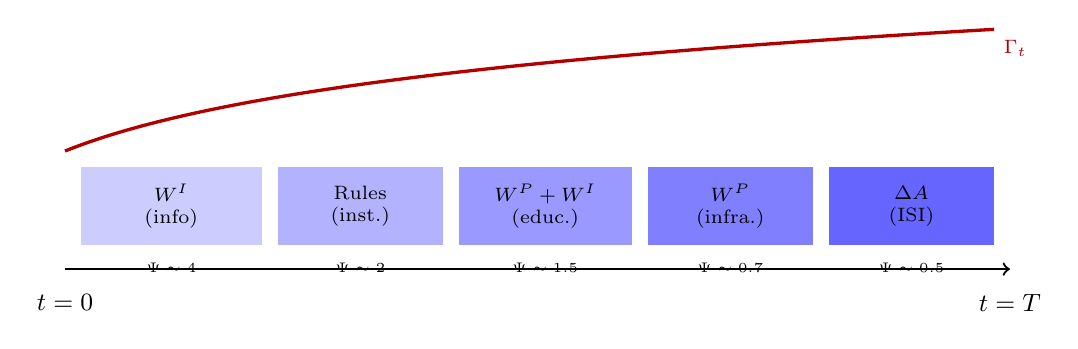
\begin{tikzpicture}[scale=1]
%% Timeline
\draw[->, thick] (0, 0) -- (12, 0);
\node[font=\small, below] at (0, -0.2) {$t=0$};
\node[font=\small, below] at (12, -0.2) {$t=T$};

%% Operators as blocks
\fill[blue!20] (0.2, 0.3) rectangle (2.5, 1.3);
\node[font=\scriptsize, align=center] at (1.35, 0.8) {$W^I$ \\ (info)};
\node[font=\tiny, below] at (1.35, 0.2) {$\Psi \sim 4$};

\fill[blue!30] (2.7, 0.3) rectangle (4.8, 1.3);
\node[font=\scriptsize, align=center] at (3.75, 0.8) {Rules \\ (inst.)};
\node[font=\tiny, below] at (3.75, 0.2) {$\Psi \sim 2$};

\fill[blue!40] (5.0, 0.3) rectangle (7.2, 1.3);
\node[font=\scriptsize, align=center] at (6.1, 0.8) {$W^P+W^I$ \\ (educ.)};
\node[font=\tiny, below] at (6.1, 0.2) {$\Psi \sim 1.5$};

\fill[blue!50] (7.4, 0.3) rectangle (9.5, 1.3);
\node[font=\scriptsize, align=center] at (8.45, 0.8) {$W^P$ \\ (infra.)};
\node[font=\tiny, below] at (8.45, 0.2) {$\Psi \sim 0.7$};

\fill[blue!60] (9.7, 0.3) rectangle (11.8, 1.3);
\node[font=\scriptsize, align=center] at (10.75, 0.8) {$\Delta A$ \\ (ISI)};
\node[font=\tiny, below] at (10.75, 0.2) {$\Psi \sim 0.5$};

%% Gamma trajectory
\draw[red!70!black, very thick, domain=0:11.8, smooth, samples=50] plot (\x, {1.5 + 0.8*ln(1+\x/2)});
\node[font=\scriptsize, red!70!black, right] at (11.8, 2.8) {$\Gamma_t$};
\end{tikzpicture}
\end{center}
\vspace{-0.5em}
\small Operators ordered by $\Psi$: highest-$\Psi$ first. The red curve shows $\Gamma_t$ rising --- steeply at first (cheap information interventions with large formation multipliers) and more gradually later (expensive industrial policy with smaller multipliers). Start soft, finish hard.
\end{vizpanel}


%% =====================================================================
\section{The Product Space as an Operator Map}
\label{ch15:sec:product_space}
%% =====================================================================

The product space (Hidalgo et al., 2007) can now be interpreted as a map of feasible operators on $W^P$.

\begin{proposition}[Product Space as Feasibility Constraint]\label{ch15:prop:product_space}
The proximity matrix $\phi_{pp'}$ (co-export probability between products) defines the feasibility of ISI operators: the probability that adding domestic production of product $p'$ succeeds is increasing in $\sum_p M_{cp}\phi_{pp'}$ (the relatedness density). Products in the dense core of the product space (machinery, chemicals, electronics) are feasible targets for economies that already produce related products. Products on the sparse periphery (minerals, agricultural commodities) offer few diversification paths.

The operator-design interpretation: the product space IS the graph of $\partial\Gamma / \partial W^P_{ij}$ for the global production network. Dense-core products have high $\partial\Gamma / \partial W^P$ because adding them creates many cross-sector linkages. Peripheral products have low $\partial\Gamma / \partial W^P$ because adding them connects to few other products.
\end{proposition}

\begin{example}[Bolivia in the Product Space]\label{ch15:ex:bolivia_ps}
Bolivia's current export basket: natural gas, zinc, gold, soy, quinoa --- all on the sparse periphery of the product space. Relatedness density to the dense core (machinery, electronics, pharmaceuticals): $\omega_{c,\text{core}} \approx 0.08$ (among the lowest in Latin America).

\textbf{Conventional ISI:} Target products adjacent in the product space --- gas processing, zinc smelting, soy flour. These increase domestic value added but do not connect to the dense core. They add edges within the peripheral block of $W^P$. $\Delta\Gamma \approx 0.02$. Modest.

\textbf{Leapfrog strategy:} Target products in the dense core --- pharmaceuticals, automotive parts, food processing machinery. These are distant in the product space (low relatedness density). The probability of success is low unless accompanied by massive human capital investment ($\mathcal{L}_{\text{HC}}$) and information rewiring ($\mathcal{L}_{\text{info}}$). But if successful: $\Delta\Gamma \approx 0.15$. Transformative.

\textbf{The sequencing solution:} (1) Information policy first: expose Bolivian engineers and technicians to the dense core (scholarships, technical exchanges, FDI in assembly operations). (2) Then education: build the capabilities (vocational training in the target sectors). (3) Then infrastructure: connect the production zones. (4) Then ISI: tariff protection for infant industries with cross-block linkages. This is the South Korean sequence, adapted to Bolivian conditions.
\end{example}


%% =====================================================================
\section{The Optimal $\Delta W$ Under Political Constraints}
\label{ch15:sec:political}
%% =====================================================================

\begin{theorem}[Politically Constrained Optimal Operator]\label{ch15:thm:political}
The optimal structural intervention under the political constraint from Chapter~14 is:
\begin{equation}\label{ch15:eq:political_optimal}
\Delta W^* = \argmax_{\Delta W \in \mathcal{F}(S^*)} \Gamma(W + \Delta W),
\end{equation}
where $S^*$ is the winning coalition and $\mathcal{F}(S^*)$ is its feasibility set. The solution differs from the unconstrained optimum because $\mathcal{F}(S^*)$ excludes structural changes that reduce any coalition member's power:
\begin{equation}\label{ch15:eq:political_constraint}
\Delta\pi_i(W, \Delta W) \geq 0 \quad \text{for all } i \in S^*.
\end{equation}

The politically constrained optimum is generically \textit{less than} the unconstrained optimum: the coalition sacrifices some $\Delta\Gamma$ to protect its members' power. The gap between constrained and unconstrained is the \textbf{political cost of structural reform}.
\end{theorem}

\begin{proposition}[The Political Cost]\label{ch15:prop:political_cost}
The political cost of structural reform is:
\begin{equation}\label{ch15:eq:political_cost}
C_{\text{political}} = \Gamma^*_{\text{unconstrained}} - \Gamma^*_{\text{constrained}} \geq 0.
\end{equation}

This cost is:
\begin{enumerate}
\item \textbf{Large when power is concentrated}: the winning coalition is small and powerful, and protecting each member's $\pi_i$ constrains the feasible $\Delta W$ severely.
\item \textbf{Small when power is equal}: the winning coalition is broad (near the grand coalition), and the political constraint is weak.
\item \textbf{Zero when the efficient $W$ also increases every agent's power}: this happens only if $W$ is already doubly stochastic (in which case no structural reform is needed) or if the reform is Pareto-improving in both allocation and power (rare).
\end{enumerate}
\end{proposition}

\begin{intuition}[Why structural reform is slow]
The political cost theorem explains why structural reform is slow even when the social returns are enormous. The unconstrained optimum might be $\Delta\Gamma = +0.20$ (a road connecting the gas enclave to the traditional economy). But the gas/government coalition blocks the road because it would reduce their power: $\Delta\pi_{\text{gas}} < 0$. The constrained optimum is $\Delta\Gamma = +0.05$ (a road that connects two urban areas, acceptable to the coalition). The gap of 0.15 is the political cost.

The only way to close the gap is to change the coalition. Chapter~14 showed that coalitions change when $\boldsymbol{\pi}$ changes. And $\boldsymbol{\pi}$ changes slowly because $W$ changes slowly (Chapter~13). The circle: $W$ is hard to change because the powerful block change $\to$ the powerful are powerful because of $W$ $\to$ $W$ is hard to change. Breaking the circle requires an exogenous shock, an information intervention that shifts preferences and coalition incentives, or the slow accumulation of cross-block edges that eventually tips the power balance.
\end{intuition}


%% =====================================================================
\section{Summary}
\label{ch15:sec:summary}
%% =====================================================================

\begin{enumerate}
\item The \textbf{operator design problem} maximizes $\Gamma$ (or $-\Var(\pi_i)$, or output multiplier) subject to a budget and row-stochasticity constraints. The first-order solution targets the edge with the largest $\partial\Gamma / \partial W_{ij}$.

\item \textbf{Five operator types}: ISI (replace foreign with domestic edges), infrastructure (physical edges), education (dual $W^P + W^I$ edges), information policy ($W^I$ only), and institutional reform (change the rules of edge dynamics).

\item \textbf{ISI that works} creates cross-block edges (modern $\leftrightarrow$ traditional). ISI that fails creates within-block edges (deepens the modern sector without connecting it). The spectral-gap criterion distinguishes them.

\item \textbf{Optimal sequencing} is $\Psi$-ordered: start with high-$\Psi$ operators (information, institutions, education) that are cheap and create the preconditions for low-$\Psi$ operators (infrastructure, industrial policy).

\item The \textbf{product space} is the operator map for $W^P$: it shows which edges are feasible (high relatedness density) and which are transformative (connect to the dense core).

\item The \textbf{political constraint} reduces the feasible $\Delta\Gamma$: the winning coalition protects its members' power. The political cost is $\Gamma^*_{\text{unconstrained}} - \Gamma^*_{\text{constrained}}$.
\end{enumerate}


%% =====================================================================
\section{Exercises}
\label{ch15:sec:exercises}
%% =====================================================================

\begin{enumerate}[label=\textbf{15.\arabic*}, leftmargin=3em]

\item \textbf{Optimal edge selection.} For a $4 \times 4$ block-diagonal $W^P$ (two blocks of 2): compute $\partial\Gamma / \partial W^P_{ij}$ for all $(i,j)$ pairs. Which edge maximizes $\Delta\Gamma$ per unit of budget? Is it within-block or cross-block?

\item \textbf{ISI-A vs.\ ISI-B.} Reproduce Example~\ref{ch15:ex:isi}: for a given budget $B = 0.10$, compute the effect on $\Gamma$, $\Var(\pi_i)$, and the Leontief multiplier of (a) adding the edge within the modern block, (b) adding the edge from modern to traditional. Which dominates?

\item \textbf{The smartphone operator.} Reproduce Example~\ref{ch15:ex:smartphone}: for a two-block economy, add $\Delta W^I = 0.05$ cross-block edges. Simulate the formation dynamics for 5 generations. Compute the steady-state $\Delta\theta$ and $\Delta x$. What is $\Psi$?

\item \textbf{Sequencing.} For a $6 \times 6$ Bolivia model (gas, urban, rural blocks), compare:
\begin{enumerate}
\item Sequence A: ISI first, then education, then information.
\item Sequence B: Information first, then education, then ISI.
\item Simulate both sequences for 10 periods. Plot $\Gamma_t$ for each. Which sequence reaches $\Gamma = 0.30$ first?
\end{enumerate}

\item \textbf{Bolivia in the product space.} Using OEC data (\texttt{oec.world}) for Bolivia:
\begin{enumerate}
\item List Bolivia's top 10 exports and their position in the product space (core vs.\ periphery).
\item Compute relatedness density to three target products: lithium batteries, food processing machinery, pharmaceutical intermediates.
\item For each target: what capability edges ($\Delta W^P$) are needed? What information edges ($\Delta W^I$)?
\item Estimate the sequencing cost for reaching each target (order of magnitude).
\end{enumerate}

\item \textbf{Hirschman vs.\ spectral gap.} For the Bolivia I-O table (from Exercise~1.7):
\begin{enumerate}
\item Compute Hirschman's backward linkages (column sums of Leontief inverse).
\item Compute $\partial\Gamma / \partial W^P_{ij}$ for all edges.
\item Do the two criteria agree on where to invest? Where do they disagree?
\item When would Hirschman's criterion lead to the wrong investment?
\end{enumerate}

\item \textbf{Political cost.} For the $N = 4$ Bolivia model: the winning coalition is $\{$Gas, Government$\}$ ($\pi_1 + \pi_2 = 0.65$). Compute (a) the unconstrained optimal $\Delta W$ and $\Gamma^*_{\text{unc}}$, (b) the constrained optimal (subject to $\Delta\pi_1 \geq 0, \Delta\pi_2 \geq 0$) and $\Gamma^*_{\text{con}}$. What is the political cost? What coalition change would reduce it?
\end{enumerate}


%% =====================================================================
\newpage
\section*{Mathematical Appendices}
\addcontentsline{toc}{section}{Mathematical Appendices}
%% =====================================================================


\subsection*{Appendix 15A: Sensitivity of $\Gamma$ to Edge Perturbations}
\addcontentsline{toc}{subsection}{Appendix 15A: Sensitivity of $\Gamma$}
\label{ch15:app:sensitivity}

\paragraph{Setup.} Let $W$ have eigenvalues $1 = \lambda_1 > |\lambda_2| \geq \cdots \geq |\lambda_N|$. The spectral gap is $\Gamma = 1 - |\lambda_2|$. We want $\partial\Gamma / \partial W_{ij}$.

\paragraph{First-order perturbation.} For a small perturbation $\Delta W$ that preserves row-stochasticity:
\begin{equation}
\Delta\lambda_k \approx \mathbf{u}_k' \Delta W \mathbf{v}_k,
\end{equation}
where $\mathbf{u}_k, \mathbf{v}_k$ are the left and right eigenvectors of $W$ for eigenvalue $\lambda_k$, normalized so $\mathbf{u}_k'\mathbf{v}_k = 1$.

For a single-edge perturbation $\Delta W_{ij} = \varepsilon$ (and $\Delta W_{i\ell} = -\varepsilon/(N-1)$ for $\ell \neq j$ to maintain row-stochasticity):
\begin{equation}
\frac{\partial\lambda_k}{\partial W_{ij}} = u_{k,i} \cdot v_{k,j} - \frac{1}{N-1}\sum_{\ell \neq j} u_{k,i} \cdot v_{k,\ell}.
\end{equation}

\paragraph{Sensitivity of $\Gamma$.} Since $\Gamma = 1 - |\lambda_2|$:
\begin{equation}
\frac{\partial\Gamma}{\partial W_{ij}} = -\text{sign}(\lambda_2)\frac{\partial\lambda_2}{\partial W_{ij}} = -\text{sign}(\lambda_2)\left[u_{2,i}v_{2,j} - \frac{u_{2,i}}{N-1}\sum_{\ell \neq j}v_{2,\ell}\right].
\end{equation}

\paragraph{Interpretation.} The sensitivity is large when $u_{2,i}$ is large (agent $i$ is important in the second left eigenvector --- she is a ``boundary'' agent between blocks) and $v_{2,j}$ is extreme (agent $j$ is at the far end of the second right eigenvector --- she is deep in one block). The optimal edge connects a boundary agent to a deep-block agent.


\subsection*{Appendix 15B: Constrained Optimization on the Stochastic Matrix Space}
\addcontentsline{toc}{subsection}{Appendix 15B: Constrained Optimization}
\label{ch15:app:constrained}

\paragraph{The constraint set.} The space of $N \times N$ row-stochastic nonnegative matrices is a convex polytope: $\mathcal{W} = \{W \geq 0 : W\ones = \ones\}$. The operator design problem is a constrained optimization on $\mathcal{W}$.

\paragraph{Projected gradient.} The gradient of $\Gamma(W)$ may point outside $\mathcal{W}$ (violating nonnegativity or row-stochasticity). The projected gradient method iterates:
\begin{equation}
W_{t+1} = \text{Proj}_{\mathcal{W}}\left(W_t + \eta \nabla_W \Gamma(W_t)\right),
\end{equation}
where $\text{Proj}_{\mathcal{W}}$ projects onto $\mathcal{W}$ by (i) setting negative entries to zero and (ii) normalizing each row to sum to 1.

\paragraph{Sinkhorn projection.} When the target is doubly stochastic (the welfare-theorems benchmark), Sinkhorn's algorithm (alternating row and column normalization) converges to the closest doubly stochastic matrix in KL-divergence.


%% =====================================================================
\subsection*{Structuralist Case Study: Tavares's ISI as Structural Engineering}
\addcontentsline{toc}{subsection}{Structuralist Case Study: Tavares (1972)}
%% =====================================================================

Maria da Concei\c{c}\~{a}o Tavares (1930--2024) was a Portuguese-born Brazilian economist who became one of the most influential structuralist thinkers of the twentieth century. Her 1972 essay ``Auge e decl\'{i}nio do processo de substitui\c{c}\~{a}o de importa\c{c}\~{o}es no Brasil'' (published in her collection \textit{Da substitui\c{c}\~{a}o de importa\c{c}\~{o}es ao capitalismo financeiro}) provided the definitive analytical autopsy of Brazilian ISI --- not as a policy failure but as a \textbf{specific operator applied to $W^P$ that succeeded at its immediate objective and failed at its structural one}.

Tavares's argument has three parts that map directly onto this chapter's framework.

\textbf{Part 1: ISI was a response to a balance-of-payments constraint, not a development strategy.} Tavares argued that Brazil's ISI was not a deliberate plan to industrialize but a ``forced march'' triggered by external bottlenecks: the Great Depression collapsed export revenues, WWII interrupted imports, and the Korean War destabilized commodity prices. Each crisis forced the domestic production of goods previously imported. In operator-design notation: each crisis was an exogenous edge destruction in $W^P_{\text{global}}$ (severed import edges), which triggered compensating edge creation in $W^P_{\text{domestic}}$ (new domestic supply chains). The ISI operator $\mathcal{L}_{\text{ISI}}$ was applied reactively, not optimally.

\textbf{Part 2: ISI created new blocks without connecting them.} The import-substitution process successfully built a modern industrial sector (automobiles, steel, chemicals, machinery). But --- and this is Tavares's crucial insight --- the new industrial sector connected primarily to \textit{itself} and to the global supply chain for capital goods, not to the pre-existing traditional economy. In operator-design terms: ISI applied $\mathcal{L}_{\text{ISI}}$ of type A (within-block), not type B (cross-block). The modern block densified internally ($W^P_{M,M}$ increased), but the edges between the modern and traditional blocks ($W^P_{M,T}$) remained dark. Pinto's structural heterogeneity was not resolved by ISI --- it was \textit{replicated at a higher level of complexity}. The tripartite economy (modern/intermediate/traditional) became a quadripartite economy (ISI-modern/export-modern/intermediate/traditional).

\textbf{Part 3: The ``decline'' of ISI was a spectral property.} Tavares showed that ISI's growth rate declined not because of ``inefficiency'' (the neoliberal critique) but because the domestic Leontief multiplier converged to a limit: once the easy substitutions were made (consumer goods, light industry), the remaining imports (capital goods, intermediate inputs) required capabilities that could only be acquired through cross-block linkages that ISI had not created. The Leontief inverse $(I - \gamma W^P)^{-1}$ had bright entries \textit{within} the modern block but dark entries \textit{between} the modern and traditional blocks. The output multiplier plateaued because the cross-block entries were near zero. In this chapter's notation: ISI maximized within-block $\Gamma$ without increasing total $\Gamma$.

\begin{center}
\begin{tabularx}{\textwidth}{LLL}
\toprule
\textbf{Tavares's argument (1972)} & \textbf{Formal object} & \textbf{This chapter} \\
\midrule
ISI as forced response to crises & Reactive $\mathcal{L}_{\text{ISI}}$, not optimal & Def.~\ref{ch15:def:isi} \\
New blocks without cross-links & ISI-A (within-block), not ISI-B (cross) & Ex.~\ref{ch15:ex:isi} \\
Structural heterogeneity replicated & $\Gamma_{\text{domestic}}$ unchanged despite new block & Prop.~\ref{ch15:prop:isi_gamma} \\
Multiplier plateau & $(I-\gamma W^P)^{-1}$ converges with dark cross-entries & Sec.~\ref{ch15:sec:product_space} \\
``Decline'' is spectral saturation & Within-block $\Gamma$ at maximum, total $\Gamma$ stagnant & Thm.~\ref{ch15:thm:optimal_edge} \\
Cross-block ISI needed & ISI-B: modern inputs from traditional sector & Ex.~\ref{ch15:ex:isi} \\
\bottomrule
\end{tabularx}
\end{center}

Tavares's essay was written in 1963 (first published) and expanded in 1972. She later served as a federal deputy in Brazil and continued to influence economic policy until her death in 2024. Her diagnosis of ISI --- that it failed not because it was wrong in principle but because it applied the operator to the wrong entries of the matrix --- remains the most precise structural analysis of Latin American industrialization. The operator-design framework of this chapter is, in a sense, the engineering manual that Tavares's diagnosis called for: given that ISI-A fails and ISI-B works, which edges should the operator target, in what sequence, and under what political constraints?


%% =====================================================================
\subsection*{Further Reading}
\addcontentsline{toc}{subsection}{Further Reading}
%% =====================================================================

\textbf{Industrial policy:} Rodrik (2004), ``Industrial Policy for the Twenty-First Century,'' CEPR Discussion Paper. Hausmann and Rodrik (2003), ``Economic Development as Self-Discovery,'' \textit{JDE}. Chang (2002), \textit{Kicking Away the Ladder}.

\textbf{The product space and structural transformation:} Hidalgo et al.\ (2007), ``The Product Space Conditions the Development of Nations,'' \textit{Science}. Hidalgo and Hausmann (2009), ``The Building Blocks of Economic Complexity,'' \textit{PNAS}. Hausmann et al.\ (2014), \textit{The Atlas of Economic Complexity}, MIT Press.

\textbf{Optimal network design:} Jackson (2008), \textit{Social and Economic Networks}, Chapter~11. For spectral methods in network design: Boyd (2006), ``Fastest Mixing Markov Chain on a Graph,'' \textit{SIAM Review}.

\textbf{The structuralist tradition on ISI:} Tavares (1972), \textit{Da substitui\c{c}\~{a}o de importa\c{c}\~{o}es ao capitalismo financeiro}, Rio de Janeiro: Zahar (the primary source). Furtado (1959), \textit{Forma\c{c}\~{a}o Econ\^{o}mica do Brasil}, Chapters~30--33. Hirschman (1968), ``The Political Economy of Import-Substituting Industrialization in Latin America,'' \textit{QJE}.

\textbf{South Korea's industrial policy:} Amsden (1989), \textit{Asia's Next Giant: South Korea and Late Industrialization}. Wade (1990), \textit{Governing the Market}. For the reciprocal control mechanisms (the state disciplines firms, not just subsidizes them): Amsden's concept maps directly to $\mathcal{L}_{\text{inst}}$ with $\delta_1$ (destruction of inefficient edges) as the enforcement mechanism.

\end{document}
